\documentclass{tufte-book}

\usepackage[T1]{fontenc}
\usepackage[utf8]{inputenc}

\usepackage{graphicx}
\setkeys{Gin}{width=\linewidth,totalheight=\textheight,keepaspectratio}
\graphicspath{{graphics/}}

\usepackage{xcolor}

\usepackage{listings}
\lstset{
	basicstyle=\ttfamily\small,
	breaklines=true,
	breakatwhitespace=true,
	xleftmargin = 0cm,
	xrightmargin = 0cm,
	framexleftmargin = 0.2em,
	frame=tb,
	literate={~} {$\sim$}{1}	% to make tilde be centered vertically
}

\usepackage{geometry}

\geometry{
	% showframe,
	paperwidth=8.5in,
	paperheight=11in,
	left=1.0in,
	%right=0.45in,
	top=0.61in,
	bottom=.61in,
	textwidth=4.3in,
	marginparsep=0.40in,
	marginparwidth=1.90in,
	includehead,
	% The text width and height are calculated automatically.
}

\usepackage{csquotes}
\usepackage[UKenglish,USenglish]{babel}

\usepackage{url}

% Used to be able to have arrows in the text
\usepackage{textcomp}	
\renewcommand{\textrightarrow}{$\rightarrow$}

\title{Delve into ESP32}
\author{Henrik Samuelsson}

\begin{document}
\maketitle

\cleardoublepage

\tableofcontents

\chapter{Introduction to ESP32}
This chapter gently introduces the ESP32 discussing what it is and what it can 
be used for.

\section{Microcontrollers}
A microcontroller unit (MCU) is a type of computer, albeit in mini format and 
with very much reduced performance compared to an ordinary desktop or laptop 
computer. Microcontrollers comes in a single integrated circuit, also known as 
a chip, and will typically be smaller than a coin.

Microcontrollers are often embedded into products and might not have 
any user interface to control them at all. They are then simply started up when 
the device is powered up and will do their work quietly behind the scenes. 
Sometimes there will be a few buttons and maybe a buzzer or a small simple 
display connected to the microcontroller that serves as an user interface.

Common usage for microcontrollers is to have them in cars, toys, white goods, 
health care equipment, audio systems, home automation systems, robots, lamps, 
cameras, power tools. This list just goes on and on. During a normal day so 
will a person be serviced by at least a dozen different microcontrollers 
without really thinking about this at all.

It is common to have more components inside the chip than just the 
microcontroller. These components will add more functionality to the chip than 
the microcontroller can provide by itself. These types of chips are often 
refereed to as system on chip (SoC) or system in package (SiP) depending on 
what technology is used when designing and manufacturing the chips.
  
\section{}

\chapter{Development Tools Setup}

This chapter discusses hardware and software needed to have to be able to do 
the exercises and projects presented in this book. The best way to learn is by 
experimenting and trying real things by yourself as opposed to just reading 
theoretical background material or watching videos.

A number of different components are required to complete all the projects 
presented in this book. If your budget is limited so will you be able to do 
many of the projects with just a handful of components, and each one is not 
really expensive either.

\section{Mandatory Hardware}\label{sec:hardware}
The following things is a must if you really want to become familiar with the ESP32.

\begin{itemize}
	\item Computer for development of software to be run on a ESP32
	\item ESP32 development kit
	\item Bread board
	\item A basic selection of passive and active electronic components
\end{itemize}

Each type of needed item is discussed more in detail in the following sections.

\subsection{Development Computer}
A computer running Linux, Windows or macOS is needed to build the software to 
be run on the ESP32. The bulk of the projects in this book have been developed 
and tested on a computer running Ubuntu 16.04, so this is the preferred 
operating system. Everything should, at least in theory, work under other o
perating system but the ride might not be as smooth.

Hardware specs on the computer are really not high. Computer to be used should 
have one or two free USB ports. There must also be some free disk space for 
software development tools. Other than that so should pretty much any computer 
work.

\subsection{ESP32 Development Kit}
A development board with an ESP32-WROOM module is considered mandatory to be 
able to test the programs that you will create. Espressif, the company behind 
the ESP32, have released a development board named ESP32-DevKitC that can be 
bought for about \$15. Do a web search and you should find several vendors that 
sell it on for example eBay or Amazon. It could also be so that your own 
favourite electronic components vendor have it in stock.

There are also various variants of the official development board developed by 
third parties. The cheapest ones can primarily be found on Chinese on-line 
market places. This can be a way to save a little money but there will usually 
be a some weeks of waiting for the order to arrive if you do not live China.

An USB cable is needed to connect the development board and your computer. 
Exact cable needed depends on the computer and what development board being 
used. USB A to micro USB is probably the type that you need. Check the ports of 
your computer and the connector on the development kit before buying.

\subsection{Bread Board}
Many of the projects requires various electronic components to be connected 
together. A fast way to hook up components is by using so called bread boards. 
Bread board comes in various colors and sizes see below picture for an example 
of a board with 830 connection points.

\begin{figure}
	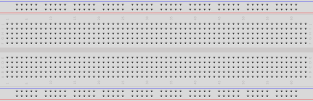
\includegraphics{bread_board.png}
	\caption[Bread board $n$.][6pt]{A common type of bread board. There are plenty of connections points and rails for dual supply voltage.}
	\label{fig:bread_board}
\end{figure}

The ESP32-DevKitC is bread board friendly and can be plugged in to the bread 
board directly. But it is fairly wide and will cover many connection points 
that we will want to have free to be able to connect other things. 
The solution is to have multiple boards connected together by the same 
principle used as when laying an jigsaw puzzle. Notice the three small knobs on 
the bottom of the board in the picture these will fit holes located at backside 
of the the top of the board. The board you want to have should be of this type 
that can be connected together with other boards. So search for a
\textquote{830 bread board} that is specified to be able to be connected
together and buy two off these boards.

An alternative is to search for ''1660 bread board`` and you will get hits were 
two bread boards are already mounted together for you on a metal plate.

Choose either one of the two options fram above but make sure that the bread
boards have gotten good reviews by other users. There are a lot of 
products out there that works less well and will cause frustration both when 
connecting the components and when running the programs that might behave 
strange if the electrical connections between are glitchy.

\subsection{Electronic Components}
A basic supply of electronic components will be needed for the projects. 
The components can be bought as separate units but it is easier and usually 
cheaper to buy a complete kit. There are starter kits, sufficient for our 
needs, that can be bought for around \$15. These kits can be found at the same 
places where you buy your ESP32 development kit. Search for 
\textquote{Arduino starter kit} or \textquote{bread board starter kit}. 
Note that the the kit does not need to contain an actual Arduino micro 
controller, the ESP32 will play the role as the controller in our projects.

The following list summarizes some of the components that should be included in 
your collection of electronic components.

\begin{itemize}
	\item Jumper wires
	\item Dupont wires
	\item An assortment of different resistors
	\item Some different ceramic and electrolytic capacitors
	\item Push buttons
	\item LED's in some different colors 
	\item Potentiometer
\end{itemize}

\section{Software}\label{sec:software}

The process of getting the ESP32 to run our own software depends on the steps and building blocks illustrated in figure~\ref{fig:software_anatomy}.

The very basic foundation of our software will be some packages that we must have on our development computer. On top of these packages so is there a library of ESP32 specific code provided by Espressif. This library is called Espressif Internet of Things Development Framework (ESP-IDF). This library abstracts away some of the hardware specific details and speeds up the development. The final piece of code that can be seen in figure~\ref{fig:software_anatomy} is labeled Our code and this will be project specific code written by us to make the ESP32 do what we want it to do.

When we are done writing a part of our code and shall test it so will we first build a binary file, this is done by running programs and scripts from a set of tools refereed to as the tool chain. A binary file will be the result of an successful build. This binary shall finally be download to a ESP32 and if we have written to code correctly so will the ESP32 start executing the code and start to behave as we intended. 

\begin{figure}
	
\includegraphics[scale=1.0]{software_anatomy.png}
	\caption[Software development $n$.][6pt]{
	Overview of the software blocks and steps needed to get an application
	running on the ESP32.
	}
	\label{fig:software_anatomy}
\end{figure}

\subsection{Software Installation}
Exact way to install the software needed to be able to build for the ESP32 depends on what operating system your development computer is running.
Only installation instructions for Ubuntu Linux is provided in this book as an illustrative example. Instructions for all supported operating systems including Ubuntu Linux can be found by searching on-line for \textquote{Espressif ESP32 installations instructions}.

Even if you choose to follow the software installations instructions that can be found on-line so is it a good idea to glance through the instructions in the sections that now follow since there are, aside from the Ubuntu specific instructions, some general useful information that is valid for all installations regardless of the underlying operating system.

\subsection{General Software Packages Installation on Ubuntu Linux}
There are, as already discussed, a number of software packages that are needed to be able to program an ESP32. Make sure that all of these are available by opening a terminal window and execute the following command.
	
\begin{lstlisting}
sudo apt-get install git
sudo apt-get install wget
sudo apt-get install make
sudo apt-get install flex
sudo apt-get install bison
sudo apt-get install libncurses5-dev
sudo apt-get install gperf
sudo apt-get install python
sudo apt-get install python-serial
\end{lstlisting}

Expected result is that the apt-get utility, a package management command line program that handles Ubuntu's Advanced Packaging Tool library, should perform installation of some new software packages.
 
Check the resulting output in the terminal for eventual problems occurring during the installation process. Should one or more packages fail to install so should you try to fix this before continuing with the next installation steps. Not having all the packages will most likely cause problems later on. Search for information on-line or post a question at the ESP32 forum that is located at www.esp32.com to resolve eventual issues.

\subsection{ESP-IDF Retrieval}

\marginnote{GitHub is a web-based Git or version control repository . It is mostly used for code. It offers all of the distributed version control and source code management functionality of Git as well as adding its own features.}

The official development framework for the ESP32 is called ESP-IDF. More or less all projects in this book will use functionality from this framework. ESP-IDF can be retrieved from GitHub and it will now be explained how to get a clone of the framework onto your development computer.

Open a terminal and move to a location where you want to store the code for the framework. It is assumed that you will create a folder named esp that will hold various sub folders for the purpose of storing ESP-IDF files. This esp folder will also later on be the parent folder for the tool chain and example projects. You can also put your your own projects for the ESP32 in this folder if you want.

\marginnote{The ESP-IDF is under active development and it could be so that there is a later release available by the time you are reading this. You can choose to get this later release instead of version 2.1. Benefits of this would be to get bug fixes and extended functionality. The down side to choosing a later release is that it may not be one-hundred percent backwards-compatible so it could break some of the code presented in this book.}

The latest current release, at the time of writing, is version 2.1. To get this release, use the following commands in a terminal.

\begin{lstlisting}
git clone \
https://github.com/espressif/esp-idf.git \
esp-idf-v2.1\ 
cd esp-idf-v2.1/
git checkout v2.1
git submodule update --init --recursive
\end{lstlisting}

\marginnote{Note that the build system does not support spaces in the path to the ESP-IDF framework. So make sure that there isn't any spaces in your path if you store the framework in some other place than suggested in the instructions.}

Expected result from these commands are the following. A new folder called esp-idf-v2.1 is created on your computer. This folder should hold various documents and folders such as for example components, docs, examples, make. The checkout command and the submodule update command ensures that the version of the ESP-IDF framework is in the same exact state as it was when release 2.1 was made.

You should now stop reading and instead write down a note of the version of ESP-IDF that you are using and where it is located on your computer. You will need this information in the next section and also later on in this book when we will setup more software tools.

\subsection{ESP-IDF Environment Path Setup on Ubuntu Linux}

\marginnote{
As before so will it only be explained here how to setup things on Ubuntu Linux. Search on-line for \textquote{Setup Path to ESP-IDF} to get information on how to proceed on other operating systems.
}

The tool chain, that eventually will build our projects, must be able to locate the ESP-IDF. This is done by setting up a an environment variable called IDF\_PATH. This variable will point at the location on your computer where you have chosen to store ESP-IDF.

Open the file \texttildelow/.profile in a text editor. The environment variable IDF\_PATH is setup by adding a line at the end of the file. Below is an example of such a line.

\marginnote{If you have /bin/bash set as login shell, and both .bash\_profile and .profile exists so should you edit .bash\_profile instead.}

\begin{lstlisting}
export IDF_PATH=~/esp/esp-idf-v2.1
\end{lstlisting}

The line you shall add should look similar but the path should  eventually be edited so that it properly reflects your particular version and location of ESP-IDF.

Save the file and close the text editor. It is then needed to logout and login again for the change to take effect.

After logging back on to the computer so can you check that the new environment variable have taken effect by the use of the following terminal command.

\begin{lstlisting}
printenv IDF_PATH
\end{lstlisting}

Expected result is that the path to the location of the ESP-IDF files is printed out in the terminal.\renewcommand{\textuparrow}{$\uparrow$}

\subsection{Tool Chain Setup on Ubuntu Linux}

\marginnote{In software development, a tool chain is a set of programming tools that are used to create a software product, which is typically another computer program or a set of related programs. In general, the tools forming a tool chain are executed consecutively so the output or resulting environment state of each tool becomes the input or starting environment for the next one.
	
Toolchain, in Wikipedia. Retrieved September 17, 2017. }

We have now got significant parts of the things that we need to be able to build our own software for the ESP32. Go back and have a look at figure~\ref{fig:software_anatomy} at page~\pageref{fig:software_anatomy} again. We have the packages and ESP-IDF now. But one of the things that are still missing is the tool chain.

The people at Espressif have provided us with a ready made tool chain for the ESP32 that we can download for free as a binary file. It is possible for more advanced user to build and tweak the tool chain by themselves. It is recommended for beginners that just want to get started as fast as possible to use the prebuilt version of the tool chain.

The exact tool chain to use is dependent on the operating system that your computer runs. This means that you shall navigate the Espressif installation instruction pages to find a tool chain for your particular operating system.

\marginnote{Direct links are generally not provided in this book. The reasoning behind this is link addresses tends to change frequently and many of the provided links would soon be broken. An attempt is instead made to present relevant search terms that should enable the reader to find the wanted resources.}

The computer used to develop the projects presented in this book runs Ubuntu Linux. Searching on line for \textquote{tool chain ESP32 download} or \textquote{xtensa-esp32-elf} and clicking around a bit on the hits for these searches will eventually lead to a download page of the correct type of tool chain.

The tool chain comes as in a packed file and we choose to extract the content in a sub folder to our already existing folder called esp. The extraction process will produce a folder called xtensa-esp32-elf in which the tool chain is located. See figure~\ref{fig:tool_chain_folder_shadowed} that visualizes the chosen file structure.

\begin{figure}
	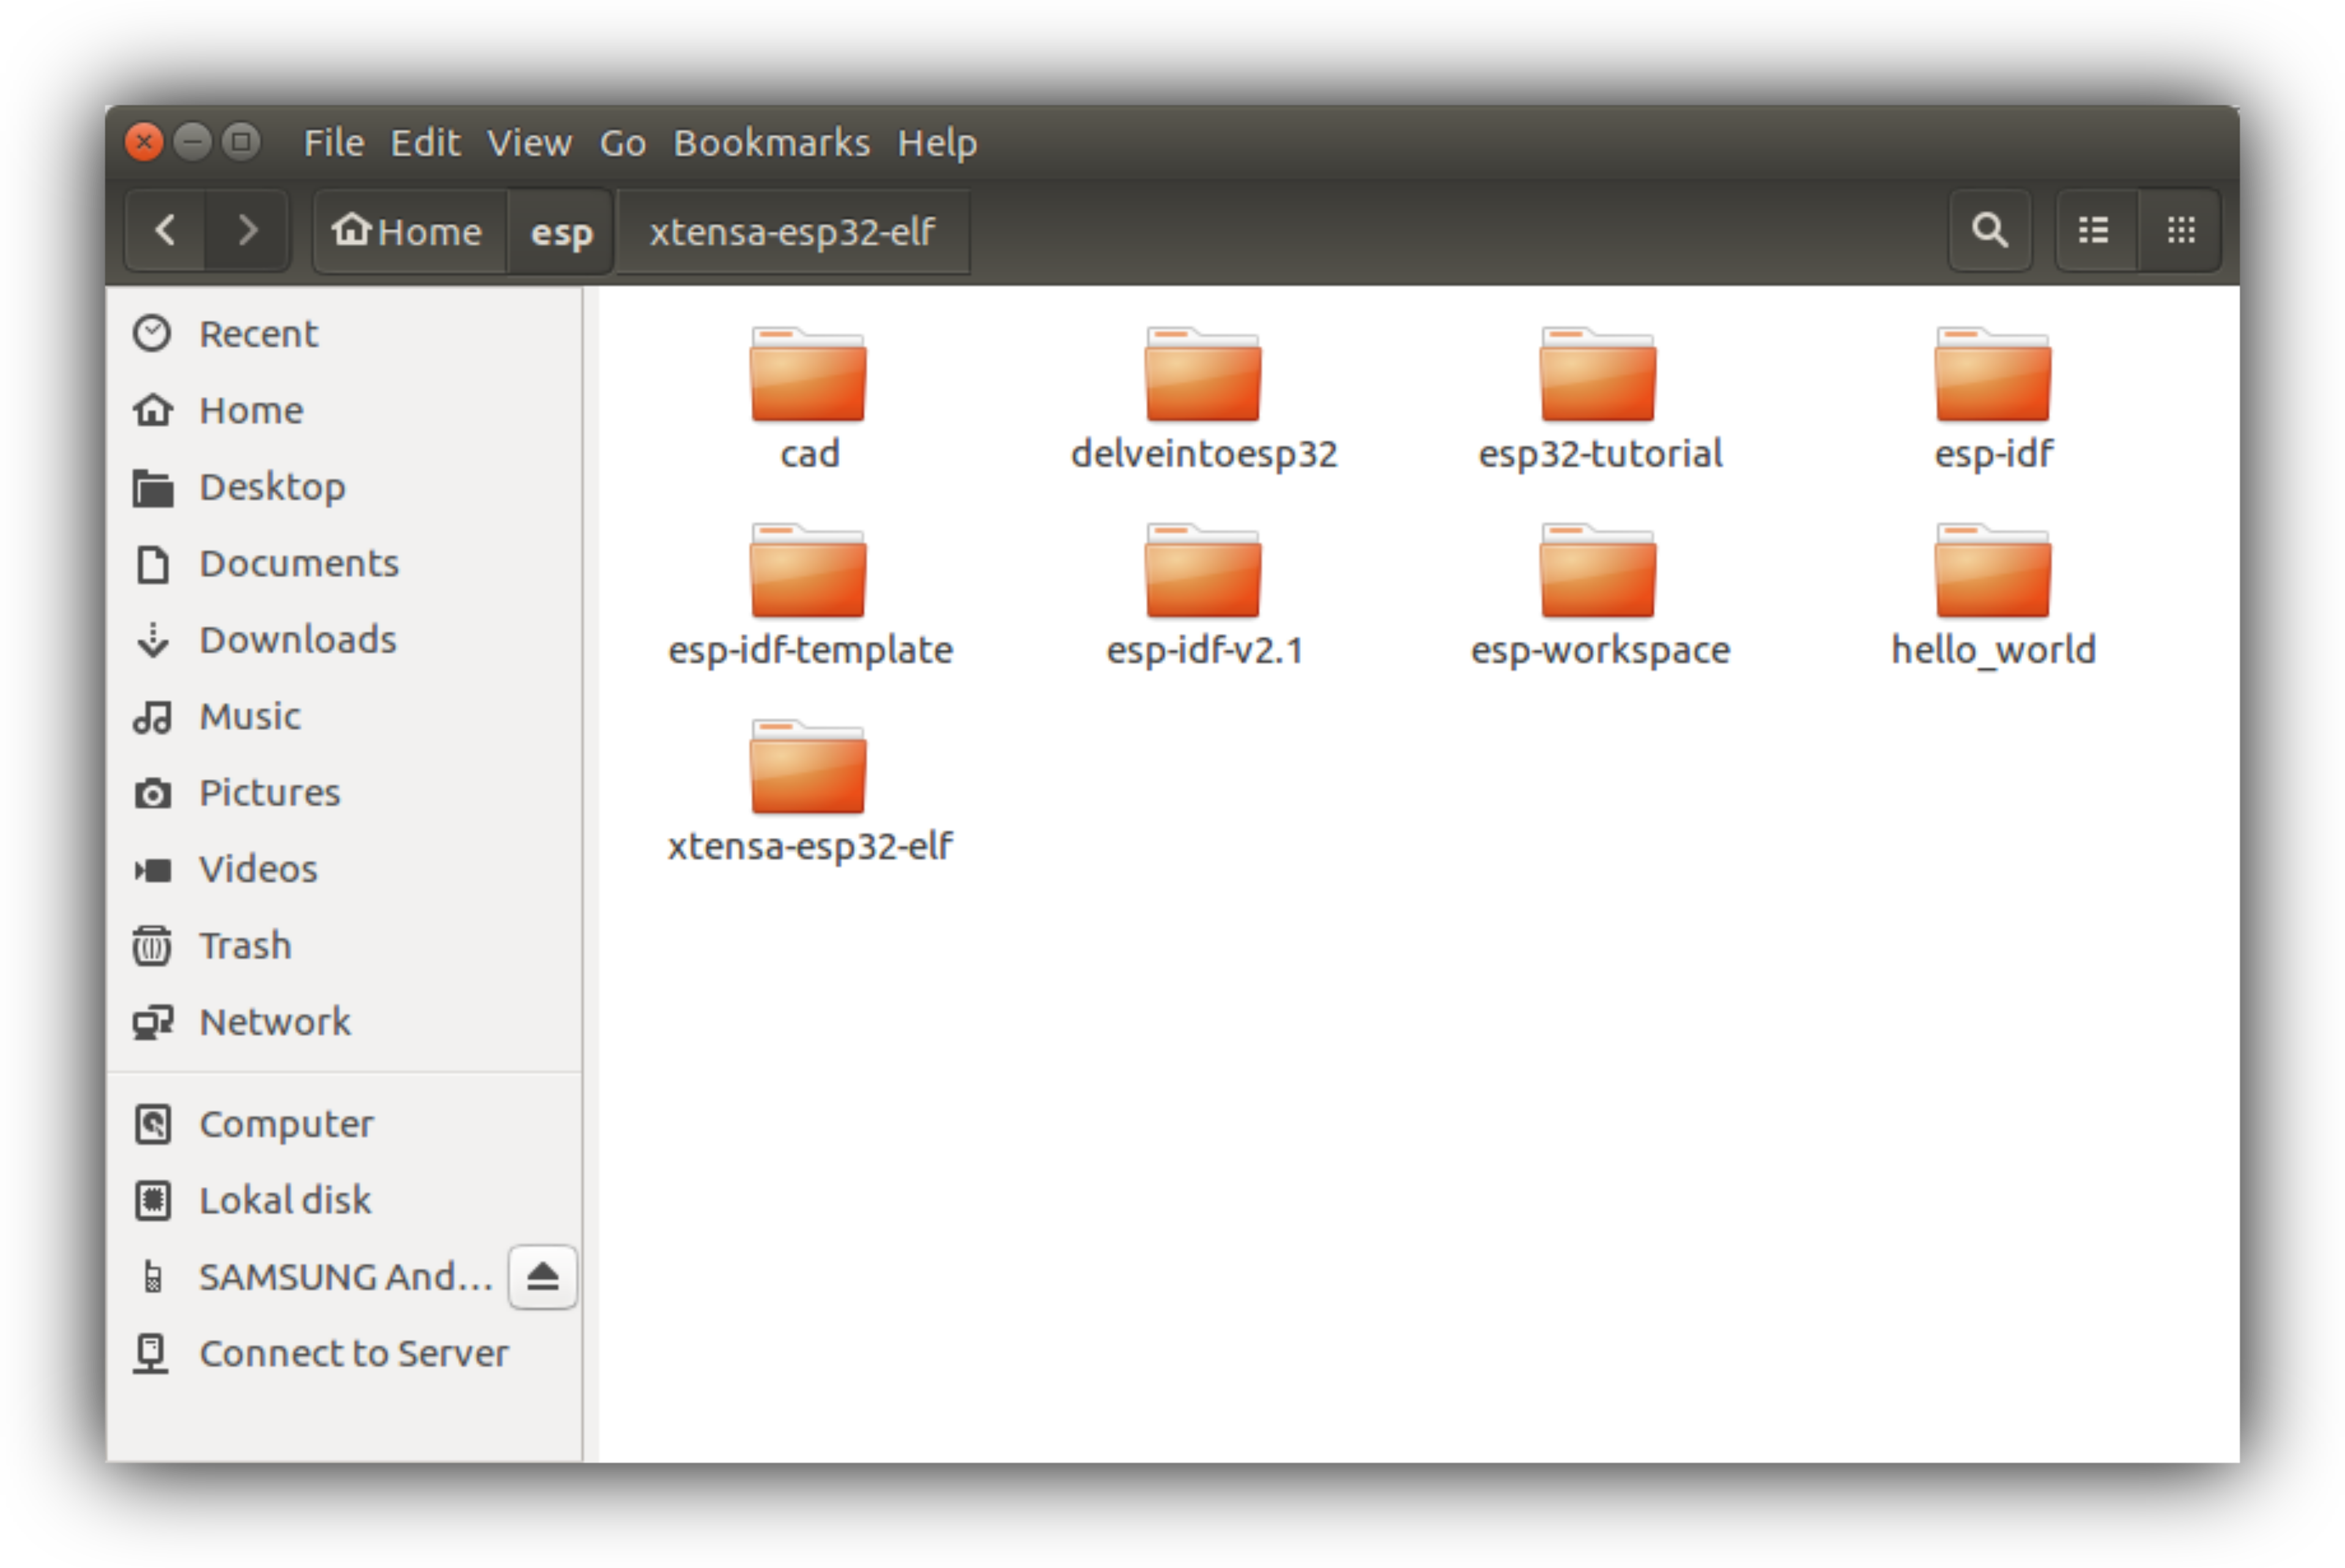
\includegraphics{tool_chain_folder_shadowed.png}
	\caption[ $n$.][6pt]{The folder xtensa-esp32-elf holds the tool chain. Both this folder and the ESP-IDF folder have been placed in a folder called esp.}
	\label{fig:tool_chain_folder_shadowed}
\end{figure}

\marginnote{If you have /bin/bash set as login shell, and both .bash\_profile and .profile exists so should you edit .bash\_profile instead.}

The development system needs to be aware of the chosen location of the tool chain. This is achieved by adding information to an environment variable called PATH. Open up the ~/.profile file and add the following line.

\begin{lstlisting}
export PATH="$PATH:$HOME/esp/xtensa-esp32-elf/bin"
\end{lstlisting}

This command will append the location of the ESP32 tool chain to the environment variable called PATH. Log out and log in again for the command to take effect. When logged in again so can the result of the change be verified by executing the following command in a terminal.

\begin{lstlisting}
printenv PATH
\end{lstlisting}

Expected result of the print environment command is that the path of the tool chain location is found at the end of the displayed string.

\subsection{Getting an Example Application}
Lets go back and have another look at figure~\ref{fig:software_anatomy} at page~\pageref{fig:software_anatomy} that illustrates what is needed to be able to build an application for the ESP32. We have the packages, a copy of the ESP-IDF framework, and the tool chain by now. The only thing that is missing before we can test to build an application is some code that makes up the actual application.

It is luckily so that there are plenty of complete example projects included in the copy of the ESP-IDF framework that we cloned previously to our computer. We will choose to test if the environment is setup correctly by building an simple application that will printout \textquote{Hello World!}.

We will build the application from the command line so start by opening up a terminal window.

\marginnote{Note that the build system does not support spaces in paths to the projects.}

Use the following commands to make a copy of the project that we will build.

\begin{lstlisting}
cd ~/esp
cp -r $IDF_PATH/examples/get-started/hello_world .
\end{lstlisting}

\subsection{Serial Port Identification} \label{sec:serial}

\marginnote{
A serial port is a communication interface through which information transfers in or out one bit at a time. Throughout most of the history of personal computers, data was transferred through serial ports to devices such as modems, terminals, and various peripherals.

While such interfaces as Ethernet and USB send data as a serial stream, the term "serial port" usually identifies hardware more or less compliant to the RS-232 standard.

Serial port, in Wikipedia. Retrieved October 14, 2017. 
}

The ESP development board will when connected to a your development computer show up as a serial port. This serial port will initially be used for transferring the program that we will build into the ESP32. The same port will additionally be used by the ESP32 to send a Hello World! message to our computer, once all the build steps are completed that is.

We will need to know the name of the serial port. The name will be different depending on type of operating system used. The name can also vary from time to time depending on what USB devices and eventual other equipment that is currently connected the computer.

The procedure for finding out the current name of the ESP32 development board is based on the following steps. First you check available serial ports when the board is not plugged in. Then you connect your board to the computer by the use of an USB cable and recheck the available serial ports. On the second check so should there be an additional new serial port. It is this port that shall be used to when transferring data between the computer and the ESP32.

How to check for available serial ports is operating system dependent. On Ubuntu Linux so are the serial ports listed by the use of the following commands.

\begin{lstlisting}
ls /dev/tty*
\end{lstlisting}

If you have a single ESP32 development board connected to a Linux computer so will its serial port most likely show up as follows.

\begin{lstlisting}
/dev/ttyUSB0
\end{lstlisting}
s
On a Macintosh computer so can the available serial ports be listed by the use of the following command.

\begin{lstlisting}
ls /dev/cu.*
\end{lstlisting}

In windows so is it for example possible to see the serial ports through the device manager. Search on-line for \textquote{How to check COM ports in Windows} if you need details for how this is done on your version of Windows.

If you have not already followed the above step for finding out the name of the serial port that can be used to communicate with your development board so shall you do that know. Take a note of the name of the port since you will need it soon.

\subsection{Setting up Serial Port Rights in Linux}
In Linux systems so must users that want to use a serial port have permission to do so. This is done by adding the logged in user to the dialout group by the use of the following command.

\begin{lstlisting}
sudo usremod -a -G dialout $USER
\end{lstlisting}

You must logout and login again for this change to take effect.

\subsection{Introduction to Menuconfig}
The ESP-IDF can be configured in different ways using a configuration utility called Espressif IoT Development Framework Configuration, also known as menuconfig.

This tool can be used to configure what components thats shall be included in the build. Having less components included that are not used leaves more room for your own application.

We shall use now use menuconfig to make sure that the Hello World project settings for the serial port is setup correctly. This will be done from a Terminal window. First navigate to the folder where you previously saved a copy of the Hello World project.

\begin{lstlisting}
cd ~/esp/hello_world
\end{lstlisting}

Now from within in this folder so shall menuconfig be run by the use of the following command.

\begin{lstlisting}
make menuconfig
\end{lstlisting}

The expected result from the above command is that a graphical user interface is started in the terminal that should look something like what can be seen in figure~\ref{fig:menuconfig_shadowed}

\begin{figure}
	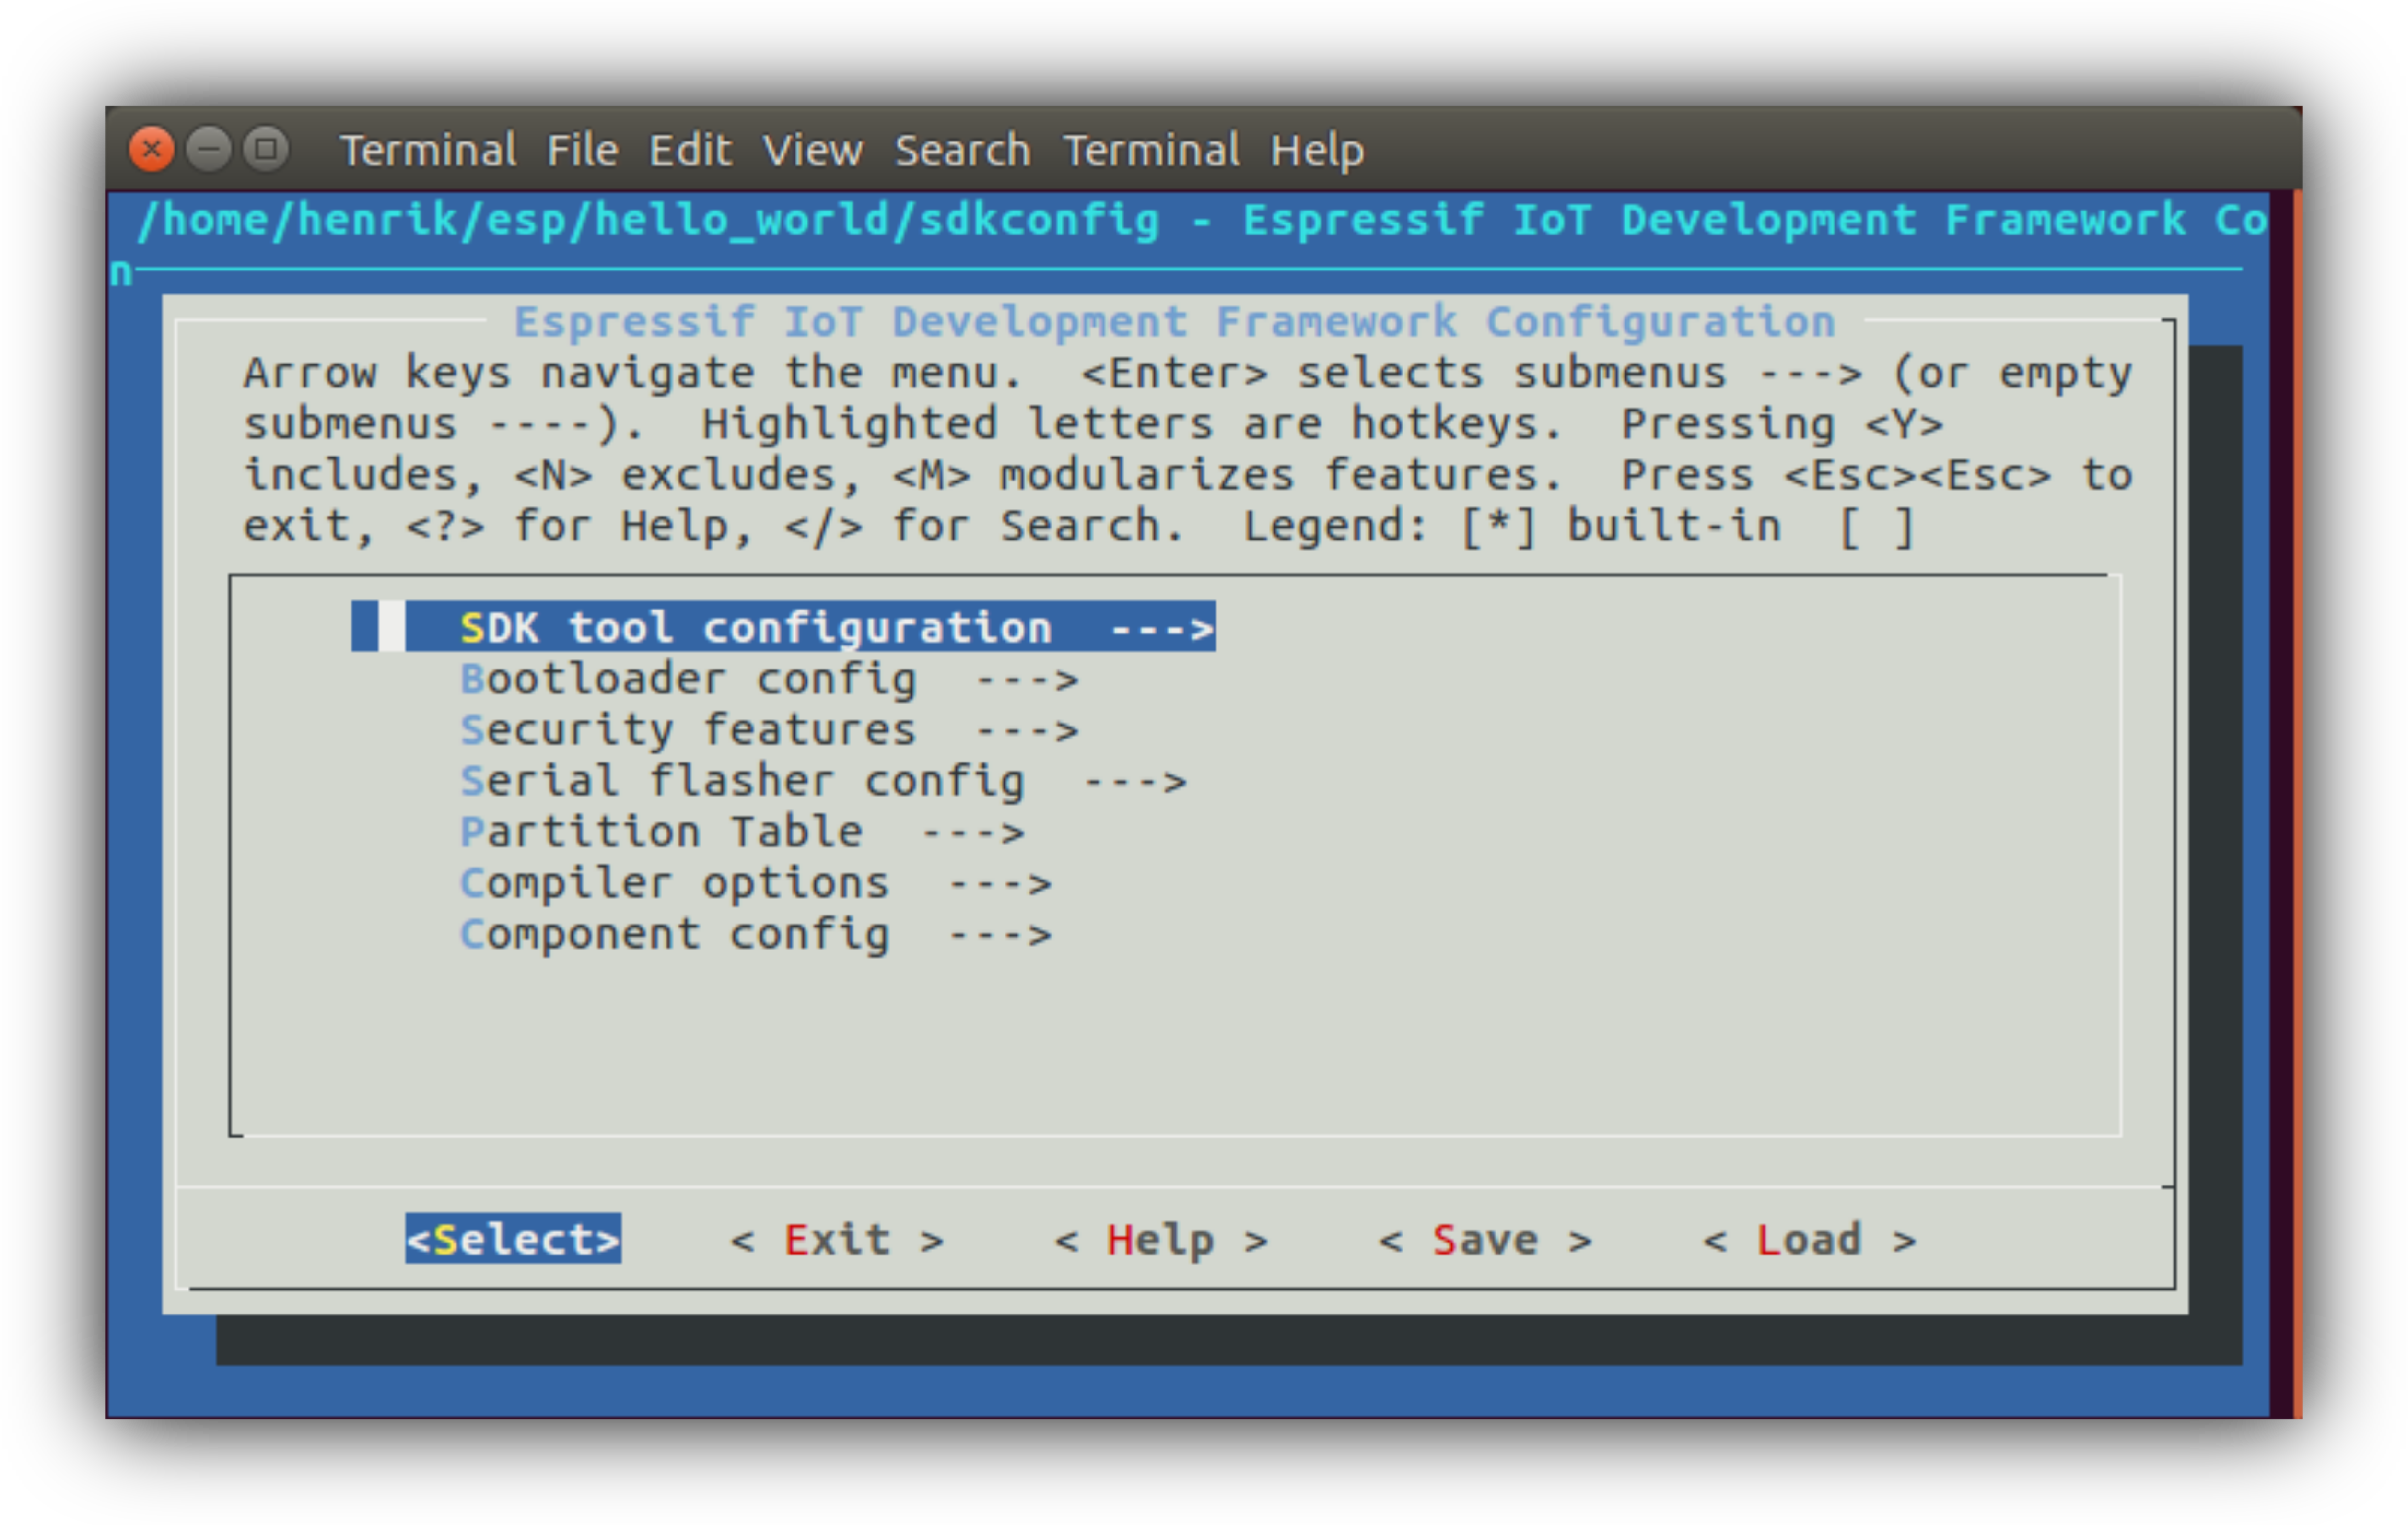
\includegraphics{menuconfig_shadowed.png}
	\caption[ $n$.][6pt]{Start view of the menuconfig tool that is used to configure the ESP-IDF framework with project specific settings.}
	\label{fig:menuconfig_shadowed}
\end{figure}

Using the mouse is not supported in menuconfig tool, navigation around among the different options in menuconfig tool is handled by the use of the keyboard. There are instructions included for how this is done in the tool itself.

\marginnote{
Not all ESP32 development boards runs at the same speed. A common speed is 40 MHz but some boards will be clocked at 26 MHz. This depends on what type of crystal that is mounted on the development board. If you get garbage as output when eventually running the Hello World project so can this be because the speed is set incorrectly. You can then try to adjust the speed in menuconfig. See Component config \textrightarrow ESP32-specific \textrightarrow ESP32\_XTAL\_FREQ\_SEL.
}
Navigate to Serial flasher config \textrightarrow Default serial port. Set this setting to the name of the serial port used for your ESP development board. Then use the save option followed by exit and you should now be back in the ordinary terminal window.

Expected result is that there now is a file called sdkconfig in your personal Hello World project folder. This is a human readable text file and if you want to double check your settings so can it be opened in a text editor. It is the flag called CONFIG\_ESPTOOLPY\_PORT in this file that controls what serial port will be used for sending down the application into the ESP32.

\subsection{Building the Application}
We have done a lot of things now good work if you have been able to follow along this far, we are almost done with the setup now.

It is time to build the actual Hello World application. You shall as before be in a terminal window and be inside the Hello World folder. Also make sure that you have your development kit connected by the USB cable so that it is powered up and ready for receiving the binary that we will soon load into the ESP32.

\marginnote{
Flash memory is a non-volatile type of memory that can be electrically erased and then written to. There is such a memory in the ESP32. Writing to this type of memory is often referred to as flashing.  
}

We will run a command that will cause both build an write of the program into to the ESP32. Execute the following command in the terminal.

\begin{lstlisting}
make flash
\end{lstlisting}

Expected result of this command is that the application is built, if this has not already been done. And then written down into to the ESP32.
The output from the command should look something like what can be seen in figure~\ref{fig:hello_world_make_flash_shadowed}

\begin{figure}
	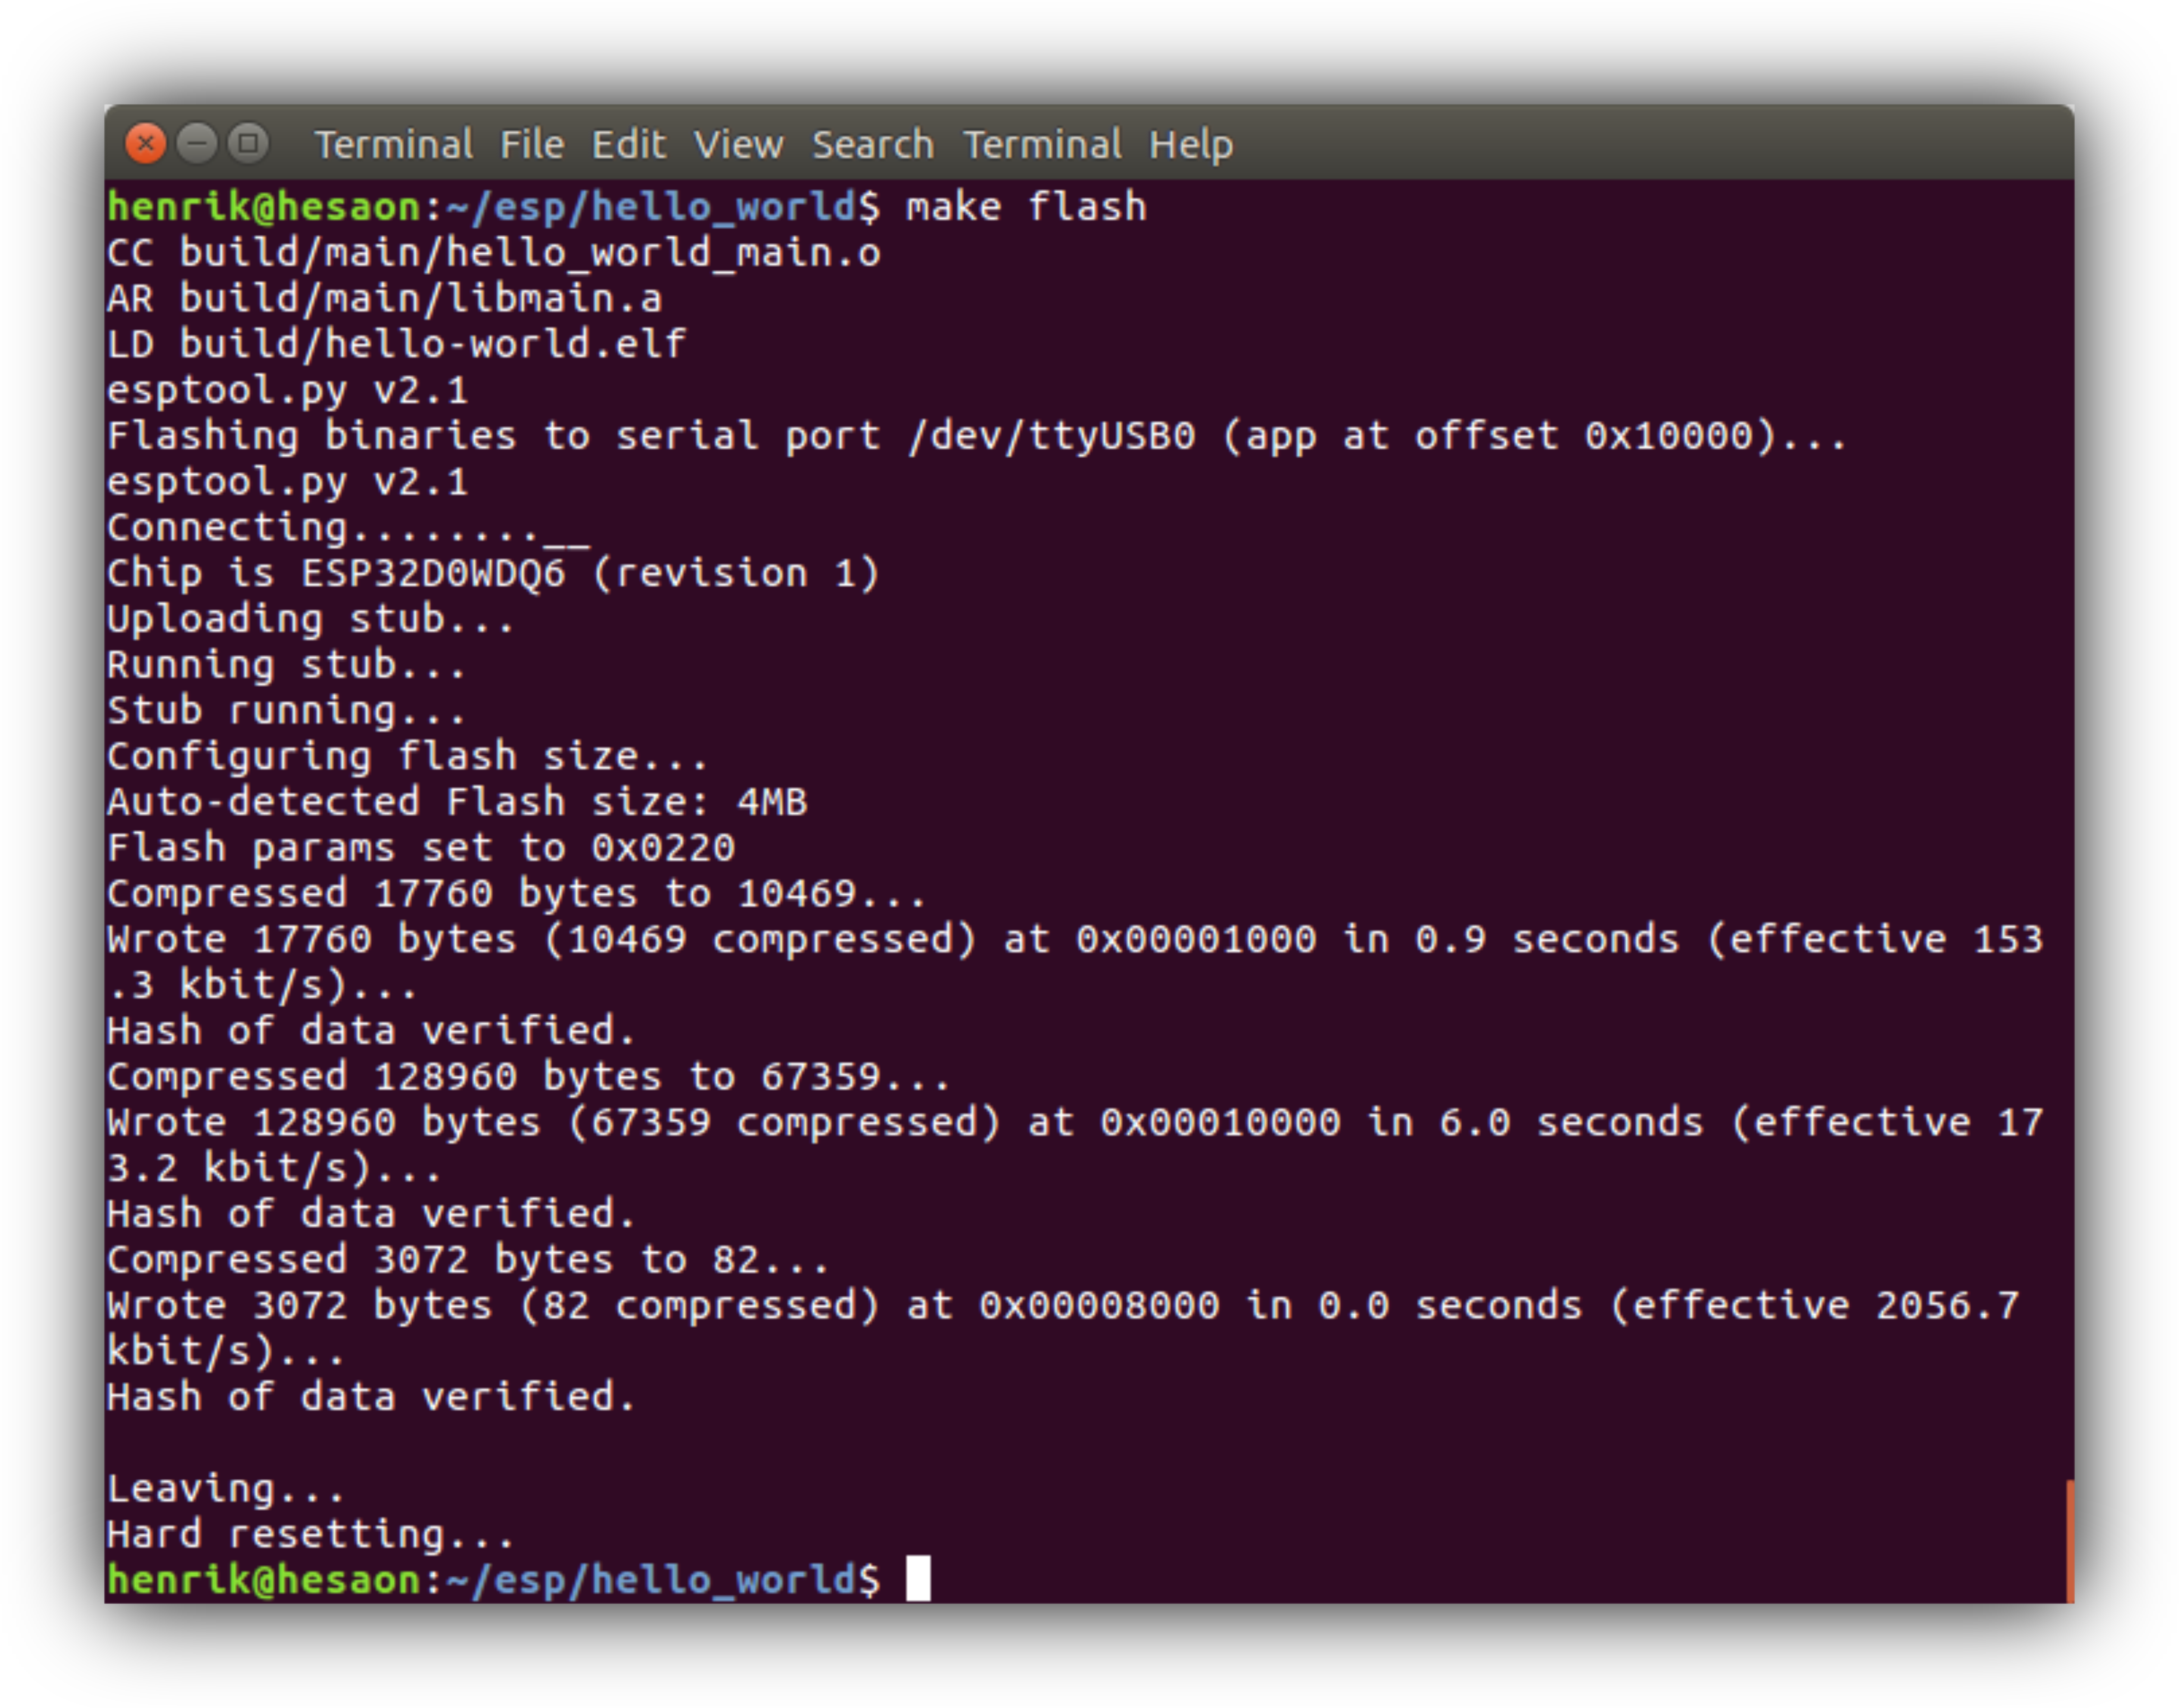
\includegraphics{hello_world_make_flash_shadowed.png}
	\caption[ $n$. ][6pt]{Screen dump from a successful build and flash procedure}
	\label{fig:hello_world_make_flash_shadowed}
\end{figure}

The code for the Hello World project should now be running in the ESP32 but nothing really seems to happen. This is because the Hello World message is printed out on the serial port and we will need to run a special terminal program on our development computer to see the output. How to do this is discussed in the next section.

\subsection{Looking at Serial Port Output}

\chapter{Setting up Eclipse}

\marginnote{
Eclipse is a very popular integrated development environment (IDE) used for computer programming. It contains a base workspace that is extensible by the use of a plug-in system. Eclipse may be used to develop applications written in many different programming languages including C and C++.
}

We have already learned how to build and download ESP32 projects using the command line. It also possible to use Eclipse to develop and build ESP32 projects.

\chapter{Bluetooth}

\end{document}
